\section{Experiments and Results}

Figure \ref{fig:gilbert2d_examples} and Figure \ref{fig:examples3d} show examples of Gilbert curves for 2D and 3D respectively.

We would like to highlight the ability of the the Gilbert curve to preserve locality analagous to the The Hilbert curve.
To do this, we create plots of average distance in embedded 2D and 3D dimension relative to the linear distance along the curve.
To allow for plot comparison, linear curve distances are normalized, the cumulative sum of average embedded distance is
used which is then modulated by the function $x^{-1-\frac{1}{d}}$.

\begin{algorithm}
  \caption{ \hskip0.5em Cumulative Binning and Data Collapse }
  \label{alg:bin_and_datacollapse}
  \begin{algorithmic}
    \State Create curve in dimension $D$, $N = |\alpha| \cdot |\beta| \cdot |\gamma|$
    \State Initialize $B = \{0\}^N$, $S = \{0\}^N$, $M=0$
    \State \textit{\# $p_i, p_j$ points in embedded dimension (2D or 3D)}
    \ForAll{ $i, j \in \{0, \dots, N\} \ \ \to p_i,p_j \in \mathbb{Z}^D$}
      \State $B_{ |i-j| } \leftarrow B_{|i-j|} + |p_i - p_j|$
      \State $M \leftarrow M + 1$
    \EndFor

    \ForAll{ $k \in \{1, \dots, N\}$ }
      \State $ x \leftarrow \frac{k}{N} $
      \State $S _ {k} \leftarrow \frac{S _ {k-1} + B _ {k}}{M}$
      \State $G ( x ) \leftarrow \frac{ S _ {k} }{ x^{1 + 1/D} }$
    \EndFor


  \end{algorithmic}
\end{algorithm}


\begin{figure}[h]
  \centering
  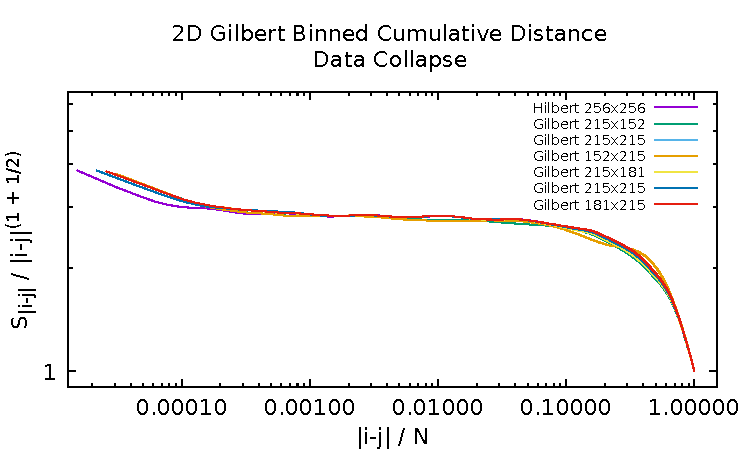
\includegraphics[width=\linewidth]{datacollapse_2d.pdf}
  \caption{ ... }
\end{figure}

\begin{figure}[h]
  \centering
  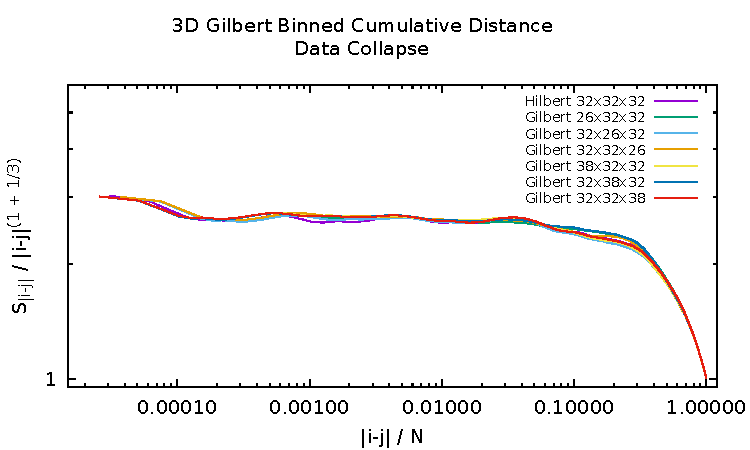
\includegraphics[width=\linewidth]{datacollapse_3d.pdf}
  \caption{ ... }
\end{figure}

\begin{figure}[h]
  \centering
  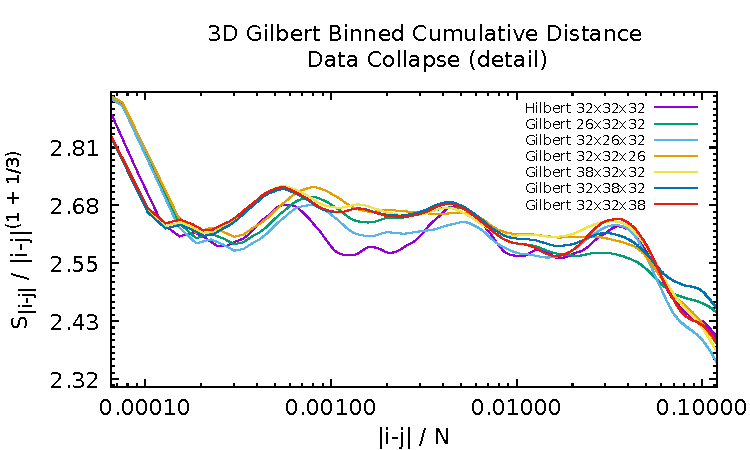
\includegraphics[width=\linewidth]{datacollapse_3d_detail.pdf}
  \caption{ ... }
\end{figure}
